\documentclass[tikz,border=1pt]{standalone} 
\usepackage{tikz}
% \usepackage{automata, arrows}
\usetikzlibrary{arrows.meta,calc,decorations.markings,math,arrows.meta}
\usetikzlibrary{positioning}
\begin{document}
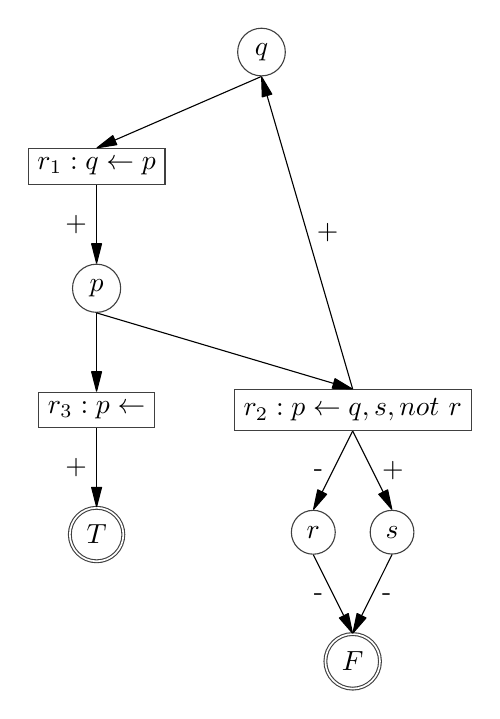
\begin{tikzpicture} [
    atom/.style={circle,  draw=black!75, minimum size=5mm},
    rule/.style={rectangle, draw=black!75, minimum size=3mm},
    sink/.style={circle, double, draw=black!75, minimum size=3mm},
    dummy/.style={midway,above},
    >={Stealth[inset=0pt,length=8pt,angle'=28,round]}
    ]
    %Nodes
    \node[atom]      (q)                                                    {$q$};
    \node[rule]      (rqp)      [below left=of q]                           {$r_1: q \leftarrow p$};
    \node[atom]      (p)        [below=of rqp]                              {$p$};
    \node[rule]      (rp)       [below=of p]                                {$r_3: p \leftarrow$};
    \node[sink]      (T)        [below=of rp]                               {$T$};
    \node[rule]      (rpqsnotr) [right=of rp]                               {$r_2: p \leftarrow q, s, not\ r$};
    \node[atom]      (r)        [below=of rpqsnotr, xshift=-.5cm]           {$r$};
    \node[sink]      (F)        [below=of r, xshift=.5cm]                   {$F$};
    \node[atom]      (s)        [below=of rpqsnotr, xshift=.5cm]            {$s$};
    %Lines
    \draw[->]       (q.south) -- (rqp.north);
    \draw[->] (rpqsnotr.south) -- (r.north) node[dummy, left] {-};
    \draw[->] (r.south) -- (F.north) node[dummy, left] {-};
    \draw[->] (rqp.south) -- (p.north) node[dummy, left] {+};
    \draw[->] (p.south) -- (rp.north);
    \draw[->] (p.south) -- (rpqsnotr.north);
    \draw[->] (rpqsnotr.north) -- (q.south) node[dummy, right] {+};
    \draw[->] (rp.south) -- (T.north) node[dummy, left] {+};
    \draw[->] (rpqsnotr.south) -- (s.north) node[dummy, right] {+};
    \draw[->] (s.south) -- (F.north) node[dummy, right] {-};
\end{tikzpicture} 
\end{document}